\chapter{Workflow and System Model}
\label{chap:model}

In this chapter, we first introduce how we extend the existing DAG model to be overhead-aware and we also describe the system model that we use in this thesis. Second we present our overhead analysis on a series of widely used workflows, which is a base of our optimization methods that will be used in simulations. Third, we introduce the experiment environments used in this thesis including FutureGrid, a distributed platform and a workflow simulator as an example of the importance of an overhead model when simulating workflow execution. The simulation of a widely used workflow verifies the necessity of taking overheads into consideration.

\section{Scientific Workflow Applications}
\label{sec:applications}

Five widely used scientific workflow applications are used in this thesis: LIGO Inspiral analysis~\cite{LIGO}, Montage~\cite{Berriman2004}, CyberShake~\cite{Graves2010}, Epigenomics~\cite{Epigenome}, and SIPHT~\cite{SIPHT}. In this section, we describe each workflow application and present their main characteristics and structures. For simplicity, system overheads are not displayed.

\paragraph{\textbf{LIGO}}
\begin{figure*}[!htb]
	\centering
	\includegraphics[width=0.45\linewidth]{figures/workflowsim/ligo_shape.pdf} \\
	\caption{A simplified visualization of the LIGO Inspiral workflow.}
	\label{fig:model_shape_ligo}
\end{figure*}
Laser Interferometer Gravitational Wave Observatory (LIGO)~\cite{LIGO} workflows are used to search for gravitational wave signatures in data collected by large-scale interferometers. The observatories' mission is to detect and measure gravitational waves predicted by general relativity (Einstein's theory of gravity), in which gravity is described as due to the curvature of the fabric of time and space. The LIGO Inspiral workflow is a data-intensive workflow. Figure~\ref{fig:model_shape_ligo} shows a simplified version of this workflow. The LIGO Inspiral workflow is separated into multiple groups of interconnected tasks, which we call branches in this thesis. However, each branch may have a different number of pipelines as shown in Figure~\ref{fig:model_shape_ligo}. 

\begin{figure*}[htb]
	\centering
	\includegraphics[width=0.4\linewidth]{figures/workflowsim/montage_shape.pdf} \\
	\caption{A simplified visualization of the Montage workflow.}
	\label{fig:model_shape_montage}
\end{figure*}

\paragraph{\textbf{Montage}}
Montage~\cite{Berriman2004} is an astronomy application that is used to construct large image mosaics of the sky. Input images are reprojected onto a sphere and overlap is calculated for each input image. The application reprojects input images to the correct orientation while keeping background emission level constant in all images. The images are added by rectifying them to a common flux scale and background level. Finally the reprojected images are co-added into a final mosaic. The resulting mosaic image can provide a much deeper and detailed understanding of the portion of the sky in question. Figure~\ref{fig:model_shape_montage} illustrates a small Montage workflow. The size of the workflow depends on the number of images used in constructing the desired mosaic of the sky. 

\begin{figure*}[htb]
	\centering
	\includegraphics[width=0.5\linewidth]{figures/workflowsim/cybershake_shape.pdf} \\
	\caption{A simplified visualization of the CyberShake workflow.}
	\label{fig:model_shape_cybershake}
\end{figure*}

\paragraph{\textbf{Cybershake}}
CyberShake~\cite{Graves2010} is a seismology application that calculates Probabilistic Seismic Hazard curves for geographic sites in the Southern California region. It identifies all ruptures within 200km of the site of interest and converts rupture definition into multiple rupture variations with differing hypocenter locations and slip distributions. It then calculates synthetic seismograms for each rupture variance, and peak intensity measures are then extracted from these synthetics and combined with the original rupture probabilities to produce probabilistic seismic hazard curves for the site. Figure~\ref{fig:model_shape_cybershake} shows an illustration of the Cybershake workflow.

\begin{figure*}[htb]
	\centering
	\includegraphics[width=0.7\linewidth]{figures/workflowsim/genome_shape.pdf} \\
	\caption{A simplified visualization of the Epigenomics workflow with multiple branches.}
	\label{fig:model_shape_genome}
\end{figure*}

\paragraph{\textbf{Epigenomics}}
The Epigenomics workflow~\cite{Epigenome} is a CPU-intensive application. Initial data are acquired from the Illumina-Solexa Genetic Analyzer in the form of DNA sequence lanes. Each Solexa machine can generate multiple lanes of DNA sequences. Then the workflow maps DNA sequences to the correct locations in a reference Genome. This generates a map that displays the sequence density showing how many times a certain sequence expresses itself on a particular location on the reference genome. A simplified structure of Epigenomics is shown in Figure~\ref{fig:model_shape_genome}. 
%Different to the LIGO Inspiral workflow, each branch in Epigenomics has exactly the same number of pipelines, which makes it more symmetric. 

\begin{figure*}[htb]
	\centering
	\includegraphics[width=0.5\linewidth]{figures/workflowsim/sipht_shape.pdf} \\
	\caption{A simplified visualization of the SIPHT workflow.}
	\label{fig:model_shape_sipht}
\end{figure*}

\paragraph{\textbf{SIPHT}}
The SIPHT workflow~\cite{SIPHT} conducts a wide search for small untranslated RNAs (sRNAs) that regulates several processes such as secretion or virulence in bacteria. The kingdom-wide prediction and annotation of sRNA encoding genes involves a variety of individual programs that are executed in the proper order using Pegasus~\cite{Deelman2004}. These involve the prediction of $\rho$-independent transcriptional terminators, BLAST (Basic Local Alignment Search Tools~\cite{BLAST}) comparisons of the inter genetic regions of different replicons and the annotations of any sRNAs that are found. A simplified structure of the SIPHT workflow is shown in Figure~\ref{fig:model_shape_sipht}. 




\begin{table}[!htb]
	\setlength{\tabcolsep}{11pt}
	\centering
	\small
	\begin{tabular}{lrrrr}
		\hline
		 & \multicolumn{1}{c}{Number} & \multicolumn{1}{c}{Average} &  \multicolumn{1}{c}{Average} \\
		Workflow	& of Tasks	 & Data Size & Task Runtime \\
		\hline
		LIGO 		&800		& 5 MB	& 228s\\
		Montage 		&300		&3 MB	&11s\\
		CyberShake 	&700		&148 MB 	& 23s\\
		Epigenomics 	&165 	& 355 MB	& 2952s\\
		SIPHT		&1000	& 360 KB 	& 180s\\
		\hline
	\end{tabular}
	\caption{Summary of the scientific workflows characteristics.}
	\label{tab:model_workflows}
\end{table} 

Table~\ref{tab:model_workflows} shows the summary of the main \textbf{workflow characteristics}: number of tasks, average data size, and average task runtimes for the five workflows. 

\section{Overhead-aware DAG Model}

A DAG models the computational activities and data dependencies within a workflow and it fits with most workflow management systems such as Pegasus \cite{Deelman2004} and DAGMan \cite{Kalayci2010}. However, the preparation and execution of a scientific workflow in distributed environments often involve multiple components and the system overheads within and between these components cannot be ignored. 
An overhead is defined as the time of performing miscellaneous work other than executing computational activities. 
To address this challenge, in this thesis, we extend the existing Directed Acyclic Graph (DAG) model to be overhead-aware (o-DAG), in which an overhead is also a node in the DAG and the control dependencies are added as directed edges. We utilize o-DAG to provide a systematic analysis of the performance of workflow optimization methods and provide a series of novel optimization methods to further improve the overall workflow performance. 


%????
%Task clustering has been widely used in optimizing scientific workflows and can achieve significant improvement in the overall runtime performance \cite{Rynge2012, Singh2008, Li2011, Cao2008} of workflows. However,  there is a lack of a generic and systematic analysis and modeling of task clustering to improve the overall workflow performance including runtime, fault tolerance, data movement and resource utilization etc. 



\begin{figure}[h!]
\includegraphics[width=0.6\linewidth]{figures/model/odag.pdf}
\centering
  \captionof{figure}{Extending DAG to o-DAG}
  \label{fig:model_odag}
\end{figure}

%In this work, we extend the DAG model to be overhead-aware (o-DAG). The reason is that system overheads play an important role in workflow execution and they constitute a major part of the overall runtime when tasks are poorly clustered. 
Fig~\ref{fig:model_odag} shows how we augment a DAG to be an o-DAG with the capability to represent scheduling overheads ($s$) such as workflow engine delay, queue delay, and postscript delay. The classification of these system overheads is based on the model of a typical workflow management system shown in Fig~\ref{fig:intro_system} and will be introduced in Section \ref{sec:overheads}. 


\section{Modeling Task Clustering}
\label{sec:task_clustering}

\begin{figure}[h!]
\centering
 \includegraphics[width=0.5\linewidth]{figures/introduction/hc.pdf}
  \captionof{figure}{An example of task clustering (horizontal clustering)}
  \label{fig:intro_hc}
\end{figure}


\begin{figure}[!htb]
\centering
 \includegraphics[width=0.5\linewidth]{figures/model/vc.pdf}
  \captionof{figure}{An example of vertical clustering.}
  \label{fig:model_vc}
\end{figure}

%Clustering delay ($c$) measures the difference between the sum of the actual task runtime and the job runtime seen by the job scheduler. The cause of clustering delay is usually the use of a job wrapper to execute a clustered job. 
%The job wrapper takes some time to extract the list of tasks and to launch them.

%With o-DAG model, we can explicitly express the process of task clustering. For example, in Fig~\ref{fig:intro_hc}, two tasks $t_2$ and $t_3$ without data dependency between them are merged into a clustered job $j_1$. Scheduling overheads ($s_3$) are reduced but clustering delay ($c_1$) is added. 

%A job ($j$) is a single execution unit and it contains one or multiple task(s). The process of merging tasks into a clustered job is called \textbf{task clustering}. 


With an o-DAG model, we can explicitly express the process of task clustering. In this thesis, we address task clustering horizontally and vertically. \textbf{Horizontal Clustering} (HC) merges multiple tasks that are at the same horizontal level of the workflow, in which the horizontal level of a task is defined as the longest distance from the entry task of the DAG to this task. \textbf{Vertical Clustering} (VC) merges tasks within a pipeline of the workflow. Tasks at the same pipeline share a single-parent-single-child relationship, which means a task $t_a$ is the unique parent of a task $t_b$, which is the unique child of $t_a$. 


Figure~\ref{fig:intro_hc} shows a simple example of how to perform HC, in which two tasks $t_2$ and $t_3$, without a data dependency between them, are merged into a clustered job $j_1$. A job is a single execution unit composed by one or multiple task(s). Job wrappers are commonly used to execute clustered jobs, but they add an overhead denoted by the clustering delay $c$. The clustering delay measures the difference between the sum of the actual task runtimes and the job runtime seen by the job scheduler. 
After horizontal clustering, $t_2$ and $t_3$ in $j_1$ can be executed in sequence or in parallel, if parallelism in one compute node is supported. In this work, we consider sequential executions only. Given a single resource, the overall runtime for the workflow in Figure~\ref{fig:intro_hc} (left) is $runtime_l= \sum_{i=1}^{4}(s_i+t_i)$, and the overall runtime for the clustered workflow in Figure~\ref{fig:intro_hc} (right) is $runtime_r=s_1+t_1+s_2+c_1+t_2+t_3+s_4+t_4$.  $runtime_l > runtime_r$ as long as $c_1 < s_3$, which is often the case in many distributed systems since the clustering delay within a single execution node is usually shorter than the scheduling overhead across different execution nodes. 


Figure~\ref{fig:model_vc} illustrates an example of vertical clustering, in which tasks $t_2$, $t_4$, and $t_6$ are merged into $j_1$, while tasks $t_3$, $t_5$, and $t_7$ are merged into $j_2$. Similarly, clustering delays $c_2$ and $c_3$ are added to $j_1$ and $j_2$ respectively, but system overheads $s_4$, $s_5$, $s_6$, and $s_7$ are removed. 



\section{System Overheads}
\label{sec:overheads}
\subsection{Overhead Classification}


\begin{figure}[h!]
	\centering
    \includegraphics[width=0.7\textwidth]{figures/model/Job_Timeline.pdf}
    \caption{Workflow Events}
    \label{fig:model_overhead}
\end{figure}


The execution of a job is comprised of a series of events as shown in Figure~\ref{fig:model_overhead} and they are defined as:
\begin{enumerate}
\item Job Release is defined as the time when the workflow engine identifies that a job is ready to be submitted (when its parents have successfully completed). 
\item Job Submit is defined as the time when the workflow engine submits a job to the local queue. 
\item Job Execute is defined as the time when the workflow engine sees a job is being executed. 
\item Task Execute is defined as the time when the job wrapper sees a task is being executed. 

\item Postscript Start is defined as the time when the workflow engine starts to execute a postscript. 
\item Postscript Terminate is defined as the time when the postscript returns a status code (success or failure). 
\end{enumerate}

Figure~\ref{fig:model_overhead} shows a typical timeline of overheads and runtime in a job. We do not specify the data transfer delay in this timeline because data transfer is handled by data transfer jobs (stage-in and stage-out jobs). 

We have classified workflow overheads into five categories as follows. 
\begin{enumerate}

\item{Workflow Engine Delay} measures the time between when the last parent job of a job completes and the time when the job gets submitted to the local queue. 
%In case of retries the value of the last retry is used for the calculation. 
The completion time of the last parent job means this job is released to the ready queue and is waiting for resources to be assigned to it. The workflow engine delay reflects the efficiency of a workflow engine (i.e., DAGMan \cite{DAGMan}). 

\item{Queue Delay} is defined as the time between the submission of a job by the workflow engine to the local queue and the time the local scheduler sees the job running. This overhead reflects the efficiency of the local workflow scheduler (e.g. Condor \cite{Frey2002}) to execute a job and the availability of resources for the execution of this job. 
%The queue delay is an estimate of the time spent in the local queue on the submit host. 

\item{Postscript Delay} is the time taken to execute a lightweight script under some execution systems after the execution of a job. Postscripts examine the status code of a job after the computational part of this job is done.

\item{Data Transfer Delay} happens when data is transferred between nodes. It includes three different types of processes: staging data in, cleaning up, and staging data out. Stage-in jobs transfer input files from source sites to execution sites before the computation starts. Cleanup jobs delete intermediate data that is no longer needed by the remainder of the workflow. Stage-out jobs transfer workflow output data to archiving sites for storage and analysis.

\item{Clustering Delay} measures the difference between the sum of the actual task runtime and the job runtime seen by the job wrapper. The cause of Clustering Delay is usually because we use a job wrapper in worker nodes to execute a clustered job that requires some delay to extract the list of tasks. 
\end{enumerate}

\subsection{Overhead Distribution}

We examined the overhead distributions of a widely used astronomy workflow called Montage \cite{Berriman2004} that is used to construct large image mosaics of the sky. Montage was run on FutureGrid \cite{Fox2013FutureGrid}. The details of FutureGrid will be introduced in Section \ref{sec:experiments}. 
Figure~\ref{fig:model_montage_queue_delay}, \ref{fig:model_montage_engine_delay} and \ref{fig:model_montage_postscript_delay} show the overhead distribution of the Montage workflow run on the FutureGrid. The postscript delay concentrates at 7 seconds, because the postscript is only used to locally check the return status of a job and is not influenced by the remote execution environment. The workflow engine delay tends to have a uniform distribution, which is because the workflow engine spends a constant amount of time to identify that the parent jobs have completed and insert a job that is ready at the end of the local queue. 
The queue delay has three decreasing peak points at 8, 14, and 22 seconds. We believe this is because the average postscript delay is about 7 seconds (see details in Figure~\ref{fig:model_montage_queue_delay} ) and the average runtime is 1 second. The local scheduler spends about 8 seconds finding an available resource and executing a job; if there is no resource idle, it will wait another 8 seconds for the current running jobs to finish, and so on. 


\begin{figure}[h!]
	\centering
    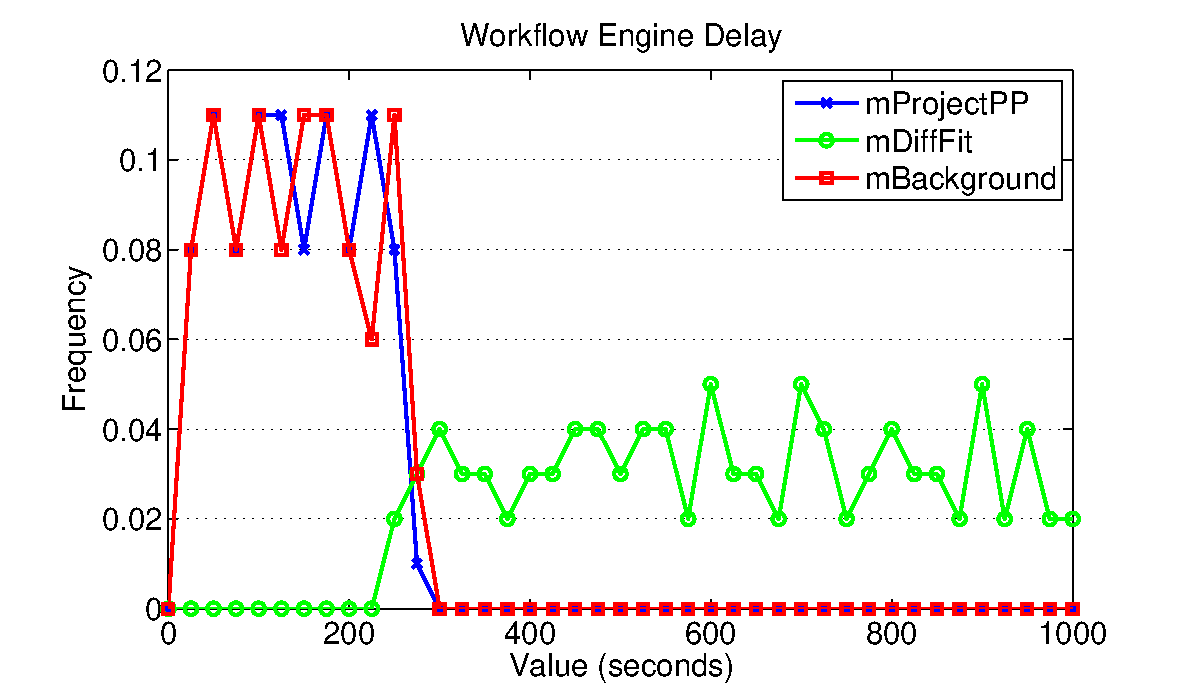
\includegraphics[height=0.4\textwidth]{figures/model/workflow_engine_delay.eps}
    \caption{Distribution of Workflow Engine Delay in the Montage workflow}
    \label{fig:model_montage_engine_delay}
\end{figure}

\begin{figure}[h!]
	\centering
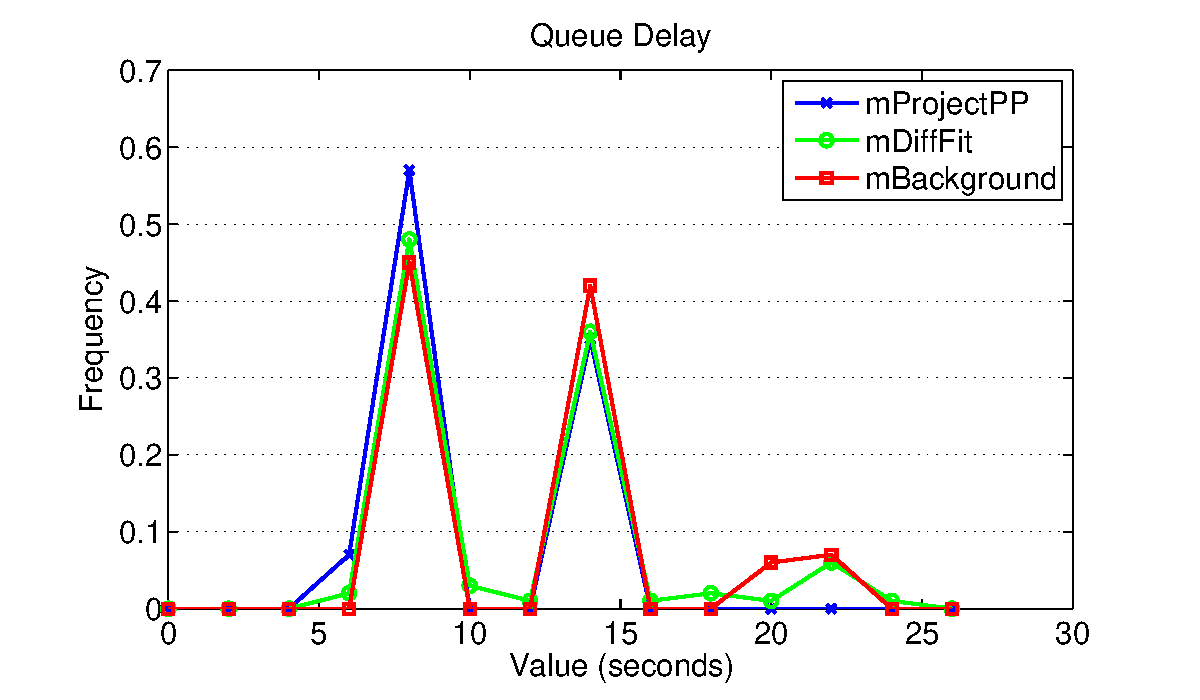
\includegraphics[height=0.4\textwidth]{figures/model/queue_delay.eps}
    \caption{Distribution of Queue Delay in the Montage workflow}
    \label{fig:model_montage_queue_delay}
\end{figure}

\begin{figure}[h!]
	\centering
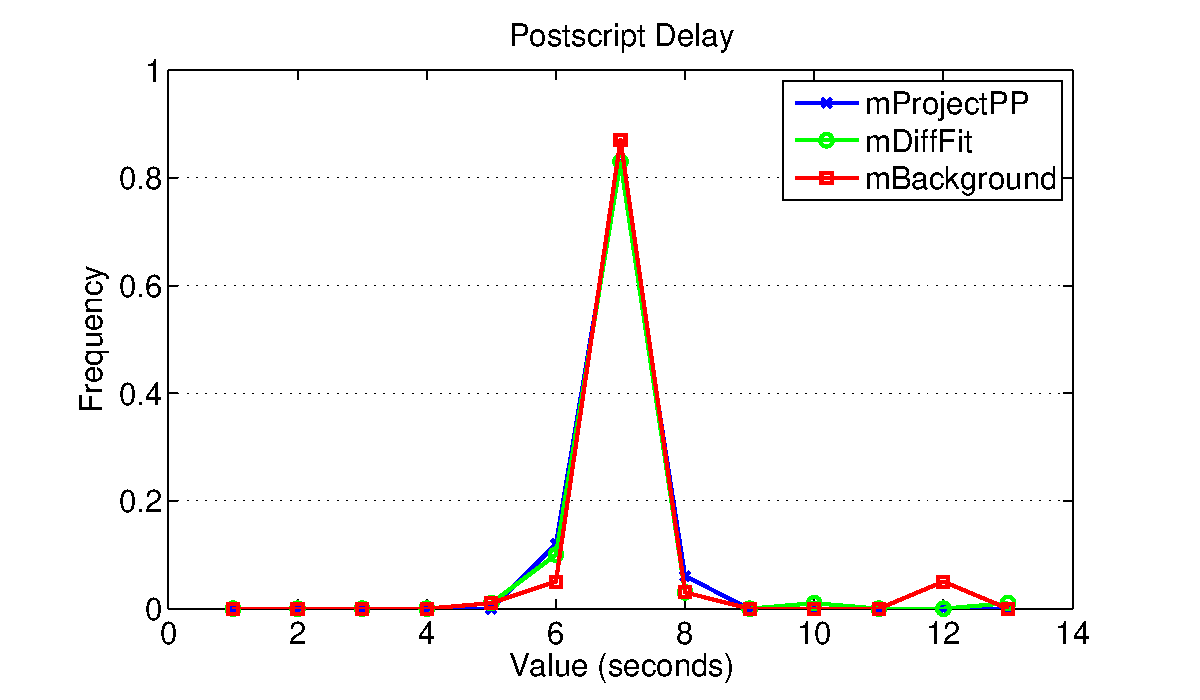
\includegraphics[width=0.7\textwidth]{figures/model/postscript_delay.eps}
    \caption{Distribution of Postscript Delay in the Montage workflow}
    \label{fig:model_montage_postscript_delay}
\end{figure}

%In our prior work \cite{Overhead2011}, we have introduced the distribution of overheads and the relationship between them. Following this, we indicate the necessity to consider the distribution of overheads rather than simply adding a constant delay after job execution. 

%Since we do not use it in ftc and btc
%We use Workflow Engine Delay as an example to show the necessity to model overheads appropriately. Figure~\ref{fig:model_montage_timeline} shows a real trace of overheads and runtime in the Montage 8 degree workflow (for visibility issues, we only show the first 15 jobs at the mProjectPP level). We can see that Workflow Engine Delay increases steadily after every five jobs. For example, the Workflow Engine Delay of jobs with ID from 6 to 10 is approximately twice of that of jobs ranging from ID1 to ID5. Figure~\ref{fig:model_montage_one_run} further shows the distribution of Workflow Engine Delay of the first 20 jobs at the mProjectPP level in the Montage workflow. After every five jobs, the Workflow Engine Delay increases by 8 seconds approximately. We call this special nature of workflow overhead as cyclic increase. The reason is that Workflow Engine (in this trace it is DAGMan) releases five jobs by default in every working cycle. Therefore, simply adding a constant delay after every job execution has ignored its potential influence on the performance.

%\begin{figure}[h!]
%	\centering
%    \includegraphics[width=0.6\textwidth]{figures/model/overhead_timeline2.pdf}
%    \caption{Workflow Overhead and Runtime. Clustering delay and data transfer delay are not shown}
%    \label{fig:model_montage_timeline}
%\end{figure}


%\begin{figure}
%\centering
%  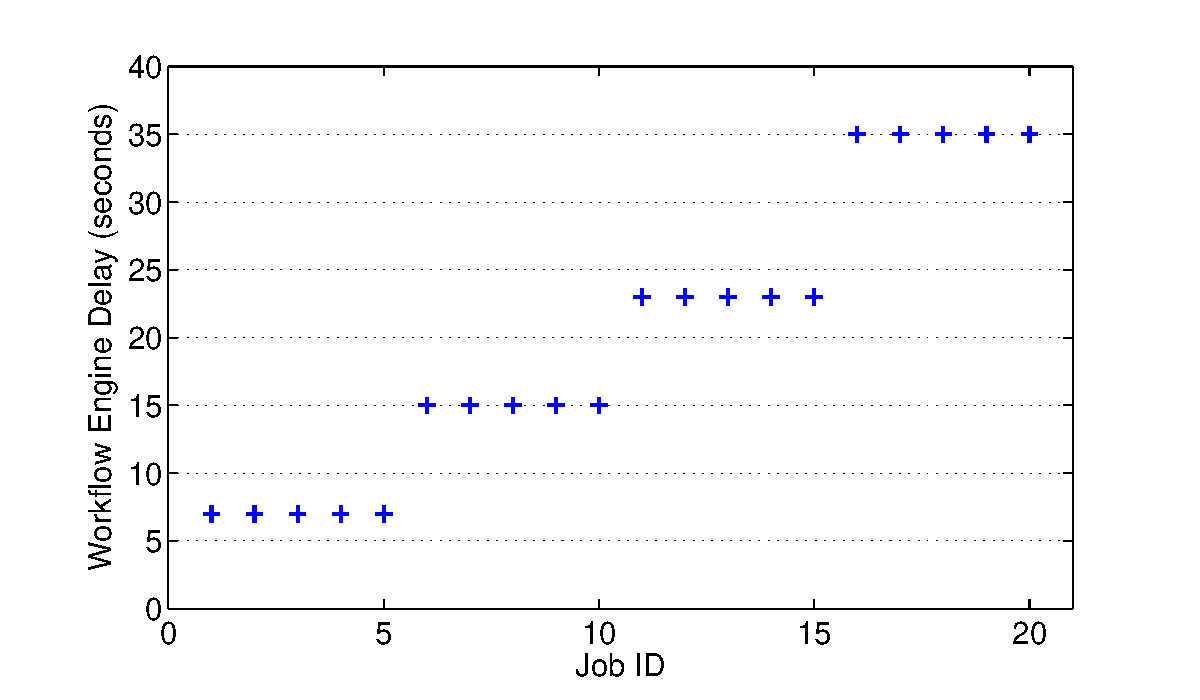
\includegraphics[width=0.7\linewidth]{figures/model/montage_one_run.eps}
%    \caption{Workflow Engine Delay of mProjectPP}
%    \label{fig:model_montage_one_run}
%\end{figure}%
\begin{figure}
  \centering
  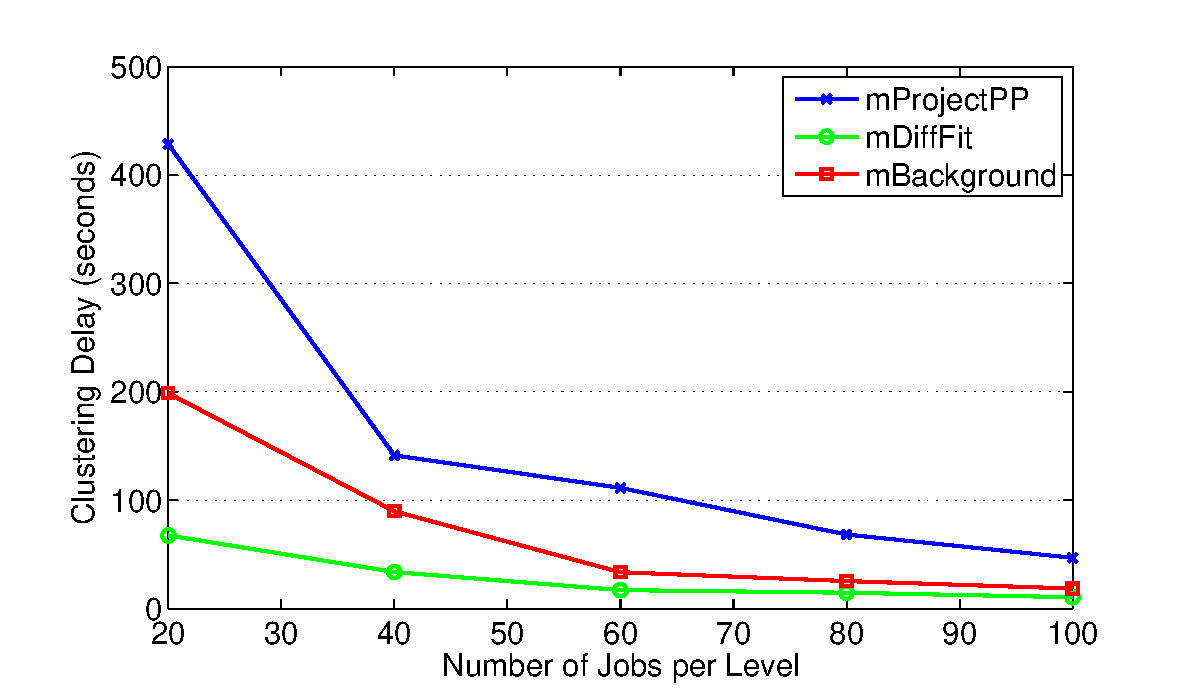
\includegraphics[width=0.7\linewidth]{figures/model/montage_clustering_delay.eps}
    \caption{Clustering Delay of mProjectPP, mDiffFit, and mBackground}
    \label{fig:model_montage_clustering}
\end{figure}





Figure~\ref{fig:model_montage_clustering} shows the average value of Clustering Delay of mProjectPP, mDiffFit, and mBackground. It is clear that with the increase of $clusters.num$ (the maximum number of jobs per horizontal level), since there are less and less tasks in a clustered job, the Clustering Delay for each job decreases. For simplicity, we use an inverse proportional model in Equation~\ref{eq:model_clustering_delay} to describe this trend of Clustering Delay with $clusters.num$. Intuitively we assume that the average delay per task in a clustered job is constant ($n$ is the number of tasks in a horizontal level). An inverse proportional model can estimate the delay when $clusters.num=i$ directly if we have known the delay when $clusters.num=j$. Therefore we can predict all the clustering cases as long as we have gathered one clustering case. This feature will be used to evaluate the performance of a workflow simulator in Section \ref{sec:experiments}. 

\begin{equation} \label{eq:model_clustering_delay}
\frac{Clustering Delay|_{clusters.num=i}}{Clustering Delay|_{clusters.num=j}}=\frac{n/i}{n/j}=\frac{j}{i}
\end{equation}




